\documentclass[a4paper,10pt]{article}

\usepackage[italian]{babel}
\usepackage[T1]{fontenc}
\usepackage[utf8]{inputenc}
\usepackage{geometry}
\usepackage{enumitem}
\usepackage{graphicx}
\usepackage{float}

\geometry{margin=1.15cm}
\setlength{\parindent}{0pt}
\setlength{\parskip}{2pt}
\setlist[itemize]{leftmargin=*,nosep}

\title{\vspace{-1.2cm}Assignment 04 -- Distributed Tic Tac Toe}
\author{Leonardo Naddei}
\date{}

\begin{document}
\maketitle
\vspace{-0.6cm}

\section{Obiettivo}
Il progetto realizza una versione distribuita del gioco del tris tramite Java
RMI. Il sistema separa l'interfaccia utente, le API remote e il motore di gioco,
in modo che client e server comunichino solo attraverso contratti espliciti.

Il gioco viene avviato quando due client effettuano la \texttt{join}. Al secondo
giocatore viene restituito il suo identificatore e il server crea un match,
gestito da un handler dedicato eseguito tramite executor con virtual thread.

\section{Architettura}
L'architettura e' decomposta in moduli indipendenti:

\begin{itemize}
      \item \textbf{clientapi}: espone la callback remota implementata dal client.
      \item \textbf{serverapi}: espone il servizio remoto implementato dal server.
      \item \textbf{client/game}: implementa il client e il loop di messaggi.
      \item \textbf{server/gameengine}: implementa matchmaking, stato del match e
            logica di avanzamento della partita.
      \item \textbf{cli}: contiene tutto l'I/O verso console tramite un renderer
            sostituibile.
\end{itemize}

\begin{figure}[H]
\centering
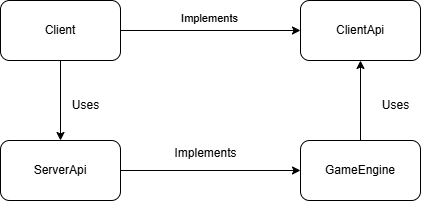
\includegraphics[width=0.72\textwidth]{modeules.png}
\caption{Diagramma dei componenti: implementazione e uso delle API remote.}
\end{figure}

\texttt{Client} implementa \texttt{ClientApi}, mentre \texttt{GameEngine}
implementa \texttt{ServerApi}. Il motore di gioco dipende inoltre da
\texttt{ClientApi} per notificare il giocatore corrente o l'esito della partita.
Questa struttura evita che client e server dipendano dalle rispettive
implementazioni concrete: entrambi conoscono solo le API remote.

\section{Algoritmo}
Durante l'analisi erano possibili due soluzioni principali. Poiche' RMI non
fornisce un supporto nativo per invocazioni asincrone, la soluzione piu'
semplice sarebbe stata un'architettura client-server con polling da parte dei
client: ogni client avrebbe interrogato periodicamente il server per sapere se
fosse il proprio turno o se la partita fosse terminata.

E' stata invece implementata un'architettura reattiva basata su notifiche. Le
invocazioni RMI non vengono usate come vere chiamate procedurali di dominio, ma
come scambi di messaggi che causano transizioni di stato nel client o nel
server. Il client invia \texttt{join} e \texttt{play}; il server invia messaggi
di callback al client tramite \texttt{receive}.

Ogni game e' associato a un handler dedicato, eseguito su un virtual thread
ottenuto dall'executor del server. Il server mantiene una coda di attesa per il
matchmaking e una mappa \texttt{Player -> Game} per instradare le giocate al
match corretto. Dentro ogni \texttt{Game} e' presente una coda producer-consumer:
\texttt{TTTServiceImpl.play} produce una \texttt{Play}, mentre
\texttt{GameHandler} consuma le mosse, aggiorna lo stato, valuta vittoria o
pareggio e invia la prossima notifica.

Il sistema puo' quindi essere letto come tre macchine a stati: una per il
servizio server/matchmaking, una per il singolo match e una per il client. Le
transizioni sono determinate dalle invocazioni RMI e dai messaggi accodati.

\section{FSM server}
La macchina a stati lato server descrive sia la fase di matchmaking sia il ciclo
del match gestito da \texttt{GameHandler}.

\begin{figure}[H]
\centering
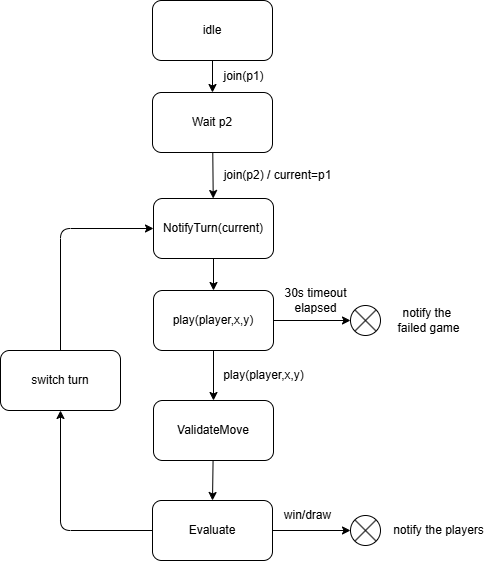
\includegraphics[width=0.82\textwidth]{serverFsm.png}
\caption{FSM lato server e handler del match.}
\end{figure}

Lo stato del match e' separato dalla logica del thread: \texttt{Game} contiene
board, giocatori, turno corrente e coda delle mosse; \texttt{GameHandler}
contiene invece il ciclo che aspetta le mosse e produce le notifiche.

\section{FSM client}
Il client e' organizzato come message loop. La callback remota
\texttt{receive(ClientMessage)} non esegue direttamente la logica applicativa:
inserisce il messaggio in una coda locale. Il thread principale del client, dopo
la \texttt{join}, resta in attesa su quella coda e reagisce ai messaggi tramite
uno \texttt{switch} sulla gerarchia sealed.

\begin{figure}[H]
\centering
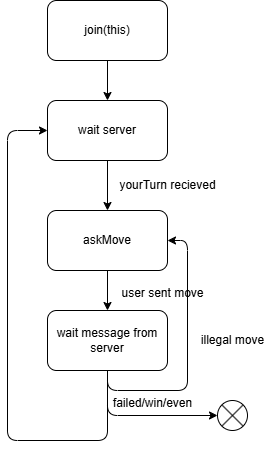
\includegraphics[width=0.72\textwidth]{clinetFsm.png}
\caption{FSM lato client basata sui messaggi ricevuti dal server.}
\end{figure}

Tutto l'I/O e' confinato nel renderer. In questo modo \texttt{ClientImpl}
contiene solo il protocollo di messaggi e puo' essere collegato a una CLI, a una
GUI o a un altro frontend senza cambiare la logica distribuita.

\section{Protocollo di messaggistica}
Il protocollo verso il client e' rappresentato da una gerarchia sealed:

\begin{itemize}
      \item \texttt{YourTurn(board)}: il server notifica al giocatore che deve
            effettuare la prossima mossa e invia la board corrente.
      \item \texttt{Won}: il giocatore ha vinto.
      \item \texttt{Lost}: il giocatore ha perso.
      \item \texttt{Even}: la partita e' terminata in pareggio.
      \item \texttt{Failed}: la partita e' fallita per errore di comunicazione,
            timeout o interruzione.
\end{itemize}

L'uso di una sealed interface rende chiuso e tipato l'insieme dei messaggi
ammessi. Il client puo' quindi gestire il protocollo con uno \texttt{switch}
esaustivo: se viene aggiunto un nuovo messaggio, il compilatore forza
l'aggiornamento dei punti in cui il protocollo viene interpretato.

Le chiamate RMI del server sono invece ridotte a due operazioni:
\texttt{join(Client)} per registrare il client e ricevere il proprio
identificatore, e \texttt{play(Player,x,y)} per inviare una mossa. Anche queste
operazioni sono usate come messaggi: \texttt{play} non valuta direttamente la
partita, ma accoda una mossa che sara' consumata dal \texttt{GameHandler}.

\section{Timeout e gestione errori}
Per evitare che un match resti bloccato indefinitamente, ogni turno ha un
timeout di 30 secondi. L'attesa della mossa viene eseguita tramite un ulteriore
task sottomesso allo stesso executor a virtual thread:
\texttt{GameHandler} attende il risultato con \texttt{Future.get(timeout)}. Se
il timeout scade, il task bloccato sulla coda viene cancellato e la partita
passa allo stato \texttt{Failed}.

Ogni errore di comunicazione durante una callback RMI viene trattato nello stesso
modo: il gioco viene rimosso dalle strutture del server e i giocatori ancora
raggiungibili ricevono \texttt{Failed}. Non e' presente un meccanismo di
heartbeat: la disconnessione viene rilevata solo quando il server prova a
notificare un client oppure quando il giocatore corrente non produce una mossa
entro il timeout.

\section{Scelte progettuali}
La scelta reattiva evita il polling e rende esplicita la direzione degli eventi:
il server notifica quando esiste qualcosa da fare, il client risponde solo quando
riceve il proprio turno. Questo riduce traffico inutile e avvicina il modello a
un sistema message passing, pur usando RMI come meccanismo di trasporto.

La separazione tra \texttt{Game}, \texttt{GameHandler}, API remote e renderer
mantiene basso l'accoppiamento. Lo stato del dominio e' confinato nel match, la
concorrenza nel game handler, il trasporto nelle API RMI e l'interazione utente
nel renderer.

\end{document}
